\documentclass{beamer}
    \usepackage{ctex}
    \usepackage{bm}
    \usepackage{hyperref}
    \usepackage{tikz}
    \usepackage{pgfplots}
    \usepackage{multirow}
    \usetikzlibrary{arrows,graphs}
    \usetikzlibrary{shapes}
    \usetheme{Antibes}
    \title{智能显示场景下的机器学习入门}
    \author{黄帅}
    \date{\today}

\begin{document}

\begin{frame}
\titlepage
\end{frame}

\section*{目录}
    \begin{frame}
        \tableofcontents
    \end{frame}

\section{介绍}
    \subsection{什么是学习}
    \begin{frame}
        \begin{block}<+->{定义}
            A computer program is said to learn from experience \textit E with respect to some class of tasks \textit T and performance measure \textit P, if its performance at tasks in \textit T, as measured by \textit P, improves with experience \textit E. (by \textit{Mitchell})
        \end{block}
        对于某类任务T和性能度量P,如果一个计算机程序在T上以P衡量的性能随着经验E而自我完善,那么我们称这个计算机程序在从经验E中学习。
        \begin{itemize}
            \item 任务T:机器学习所关注的任务是人类很难通过总结具体规则进行解决的任务。
            \item 性能度量P:为了可以量化地衡量机器学习算法的表现,通常根据不同的任务类型设计相应的性能度量方式。
            \item 经验E:根据学习过程中获取到的经验种类,机器学习可以分为\textit{有监督学习}和\textit{无监督学习}两大类。
        \end{itemize}
    \end{frame}

    \begin{frame}
        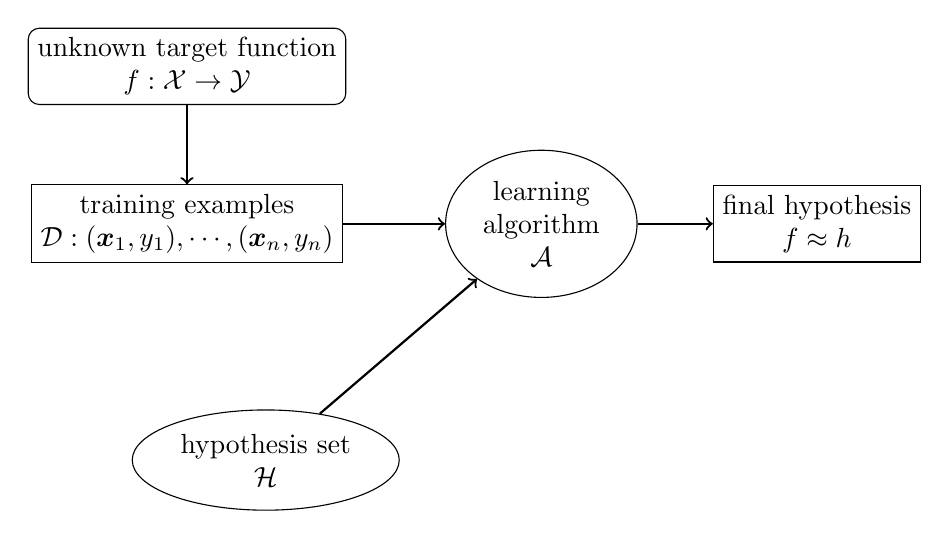
\begin{tikzpicture}
            \node (n1) at (0,0)[draw,rectangle,rounded corners,align=center]{unknown target function \\ $f:\mathcal X \to \mathcal Y$};
            \node (n2) at (0,-2)[draw,rectangle,align=center]{training examples \\ $\mathcal D:(\bm x_1, y_1),\cdots,(\bm x_n, y_n)$};  
            \node (n3) at (4.5,-2)[draw,ellipse,align=center]{learning\\algorithm\\ $\mathcal A$};
            \node (n4) at (8,-2)[draw,rectangle,align=center]{final hypothesis \\ $f\approx h$};
            \node (n5) at (1,-5)[draw,ellipse,align=center]{hypothesis set \\ $\mathcal H$};
            \draw [thick,->] (n1)--(n2);
            \draw [thick,->] (n2)--(n3);
            \draw [thick,->] (n3)--(n4);
            \draw [thick,->] (n5)--(n3);
        \end{tikzpicture}
    \end{frame}

\section{线性模型}
    \subsection{线性回归}
    \begin{frame}
        给定数据集$D=\{(\bm x_1,y_1),(\bm x_2,y_2),\cdots,(\bm x_m,y_m)\}$,其中$\bm x_i=(x_{i1};x_{i2};\cdots;x_{id}),y_i\in\mathbb R$。

        ``线性回归''(linear regression)试图学得
        \begin{block}<+->{模型定义}
            $$f(\bm x)=\bm{w}^T\bm{x}+b\,\text{使得}\, f(\bm x_i)\approx y_i$$
        \end{block}
        其中,$\bm x$是样本中提取出的特征向量;$\bm w$和$b$是待学习参数。
        \begin{itemize}
            \item 任务T:回归问题,预测连续值$y_i$
            \item 性能度量P:均方误差$\frac{1}{m}\sum_{i=1}^m(y_i-\bm w\bm x_i)^T(y_i-\bm w\bm x_i)$
            \item 经验E:权重参数$w_i$
        \end{itemize}
    \end{frame}
    \begin{frame}
    优化过程为:令$$\hat{\bm w}=(\bm w;b)$$$$\bm X=\left[\begin{matrix}x_{11}&x_{12}&\cdots&x_{1d}&1\\x_{21}&x_{22}&\cdots&x_{2d}&1\\\vdots&\vdots&&\vdots&\vdots\\x_{m1}&x_{m2}&\cdots&x_{md}&1\end{matrix}\right]$$
    对应的标记也写成向量形式$$\bm y=(y_1;y_2;\cdots;y_m)$$
    则优化目标为
    $$\hat{\bm w}^\ast=\mathop{\arg\min}_{\hat{\bm w}}(\bm y-\bm X\hat{\bm w})^T(\bm y-\bm X\hat{\bm w})$$
    令$E_{\hat{\bm w}}=(\bm y-\bm X\hat{\bm w})^T(\bm y-\bm X\hat{\bm w})$,对$\hat{\bm w}$求导得:
    $$\frac{\partial E_{\hat{\bm w}}}{\partial\hat{\bm w}}=2\bm X^T(\bm X\hat{\bm w}-\bm y)$$
    \end{frame}
    \begin{frame}
        如果$\bm X^T\bm X$为正定矩阵,那么有
        $$\hat{\bm w}^\ast=(\bm X^T\bm X)^{-1}\bm X^T\bm y$$
        对应的线性回归模型为
        $$f(\hat{\bm x_i})=\hat{\bm x}_i^T(\bm X^T\bm X)^{-1}\bm X^T\bm y$$
        Q:如果$\bm X^T\bm X$不是正定矩阵?会有多个解,此时由模型的\href{http://blog.csdn.net/u011938325/article/details/75173140}{\textbf{归纳偏好}}决定采用哪个解,常见的做法是引入\href{https://www.zhihu.com/question/20924039}{\textbf{正则化项}}。
    \end{frame}

    \subsection{对数几率回归}
    \begin{frame}
        如果要做的是分类任务应该怎么办?只需要找一个单调可微函数将分类任务的真实标记$y$与线性回归模型的预测值联系起来.
        \begin{block}<+->{对数几率回归模型}
            \begin{equation*}
                f(\bm x)=\frac{1}{1+e^{-(\bm w^T\bm x+b)}}
            \end{equation*}
            其中,$\bm x$是样本中提取出的特征向量;$\bm w$和$b$是待学习参数。
        \end{block}
        对数几率回归又称\textit{Logistic Regression},虽然名字中带着回归两个字,但它是一个分类模型。
        \begin{itemize}
            \item 任务T:分类任务
            \item 性能度量P:准确率(精准率,召回率)
            \item 经验E:权重参数$w_i$
        \end{itemize}
    \end{frame}
    \begin{frame}
        \begin{center}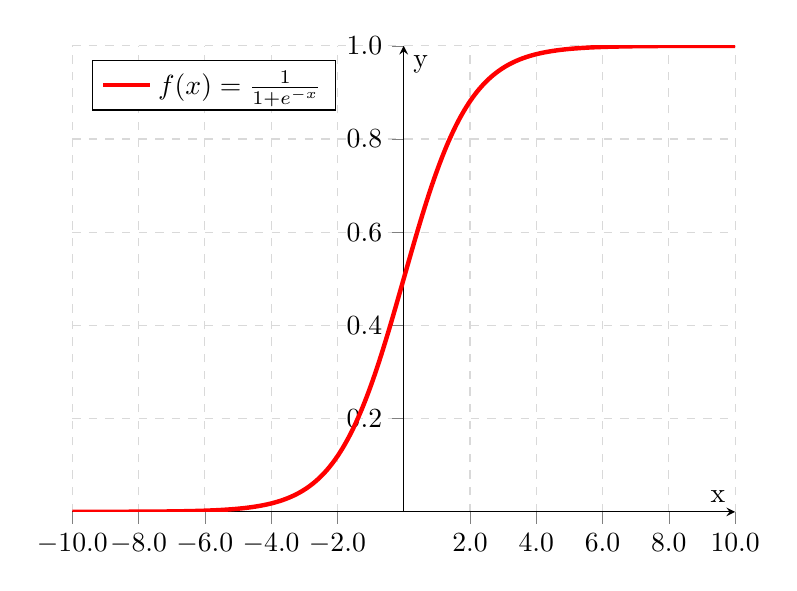
\begin{tikzpicture}
            \begin{axis}[
                legend pos=north west,
                axis x line=middle,
                axis y line=middle,
                x tick label style={/pgf/number format/fixed,
                                    /pgf/number format/fixed zerofill,
                                    /pgf/number format/precision=1},
                y tick label style={/pgf/number format/fixed,
                                    /pgf/number format/fixed zerofill,
                                    /pgf/number format/precision=1},
                grid = major,
                width=10cm,
                height=7.5cm,
                grid style={dashed, gray!30},
                xmin=-10,     % start the diagram at this x-coordinate
                xmax= 10,    % end   the diagram at this x-coordinate
                ymin= 0,     % start the diagram at this y-coordinate
                ymax= 1,   % end   the diagram at this y-coordinate
                %axis background/.style={fill=white},
                xlabel=x,
                ylabel=y,
                tick align=outside,
                enlargelimits=false]
              % plot the stirling-formulae
              \addplot[domain=-10:10, red, ultra thick,samples=5000] {1/(1+exp(-x))};
            %   \addplot[domain=-1:1, blue, ultra thick,samples=500] {1/(1+exp(-10*x))};
              \addlegendentry{$f(x)=\frac{1}{1+e^{-x}}$}
            %   \addlegendentry{$g(x)=\frac{1}{1+e^{-10x}}$}
            \end{axis}
        \end{tikzpicture}\end{center}
    \end{frame}
    \begin{frame}
        由定义可得,$$\ln\frac{y}{1-y}=\bm w^T\bm x+b$$
        其中,$\frac{y}{1-y}$被称为\textbf{几率},反映了样本$\bm x$作为正例的相对可能性.对几率取对数则得到\textbf{对数几率}.

        如何求取参数$\bm w,b$?
    设\begin{equation*}\begin{split}
    p(y=1|\bm x)&=\frac{e^{\bm w^T\bm x+b}}{1+e^{\bm w^T\bm x+b}}\\
    p(y=0|\bm x)&=\frac{1}{1+e^{\bm w^T\bm x+b}}
    \end{split}\end{equation*}
    通过极大化对数似然$$\mathcal L(\bm w,b)=\sum_{i=1}^m\ln p(y_i|\bm x_i;\bm w,b)$$求取相应的参数$(\bm w,b)$.
    \end{frame}

    \subsection{性能度量}
    \begin{frame}
        \begin{center}\begin{tabular}{|c|c|c|}
            \hline
            \multirow{2}{*}{真实情况} &
            \multicolumn{2}{c|}{预测结果}\\
            \cline{2-3}
              & 正例 & 反例 \\
            \hline
            正例 & TP(真正例) & FN(假反例) \\
            \hline
            反例 & FP(假正例) & TN(真反例) \\
            \hline
            \end{tabular}\end{center}
        \begin{itemize}
            \item 精准率(查准率)$$P=\frac{TP}{TP+FP}$$
            \item 召回率(查全率)$$R=\frac{TP}{TP+FN}$$
        \end{itemize}
    \end{frame}

\section{应用举例}
    \subsection{Kaggle竞赛 - Titanic}
    \begin{frame}
    \end{frame}

\section{学习材料}
    \begin{frame}
        \href{https://github.com/ShuaiHuang/Machine-Learning-Material}{GitHub Repository}
    \end{frame}

\end{document}